\documentclass[10pt,a4paper]{article}
\usepackage[T1]{fontenc}
\usepackage[utf8]{inputenc}
\usepackage{lmodern}
\usepackage{microtype}
\usepackage[margin=2.1cm]{geometry}
\usepackage{amsmath,amssymb}
\usepackage{booktabs}
\usepackage{tabularx}
\usepackage{xltabular}
\usepackage{flafter}
\usepackage{graphicx}
\usepackage{enumitem}
\usepackage{xcolor}
\usepackage[colorlinks=true,linkcolor=black,citecolor=black,urlcolor=blue!50!black]{hyperref}
\usepackage{caption}
\captionsetup{font=small,labelfont=bf}

\setlist{nosep,leftmargin=1.4em}
\newcolumntype{L}{>{\raggedright\arraybackslash}X}
\newcommand{\PR}{\mathrm{PR}}
\newcommand{\T}{\mathbb{T}^2}
\newcommand{\dT}{d_{\mathbb{T}}}
\newcommand{\verdict}[1]{\textbf{#1}}
\setlength{\parskip}{3pt}
\setlength{\parindent}{0pt}

\title{\vspace{-1.6cm}\large\textbf{``What Does a Game-Trained Embedding Learn?'' (draft of 8 Oct 2026)}\\
\normalsize Summary of the paper as it stands, and the review comments that matter}
\author{}
\date{}

\begin{document}
\maketitle
\vspace{-2.2cm}
\begin{center}\small\parbox{0.9\textwidth}{\centering Prepared for P.\ Sole-Vilaro and coauthors, 26 Oct 2026. Every number comes from the reproduction bundle or from the 120-run baseline ensemble (R1) in \texttt{rev2/}; the full assessment and run plan are in \texttt{REVISION\_PLAN.md}.}\end{center}

\section*{1. The paper in brief}

The paper takes the multi-head architecture of Taranc\'on-\'Alvarez et al.\ (2026), which embeds a family of PDE solutions in a shared latent curve read by per-instance linear heads, and trains it by adversarial self-play on a pursuit--evasion game on the flat torus. It then asks what the latent space of the trained network encodes. The answer is organised around separating two objects: the \emph{strategy ensemble} (the heading curves the heads output, one per evader initial condition), which game theory constrains, and the \emph{latent curve} $\boldsymbol{H}(t)$ upstream of the heads, which it does not. The main claims are (i) the ensemble is low-rank, as the constant-heading saddle predicts, and this rank is selected by training rather than built in; (ii) the latent curve carries a larger ``overhead'' that no head reads and that is attributable to the input featurisation; (iii) the game's topology appears as clusters in control space, not as latent dimensions; (iv) a tempting pursuer--evader spectral asymmetry does not survive a symmetrised-training control. A self-play protocol study (\S8) and a value-level check against an independently trained HJI critic (\S9) complete the draft. Every claim has a named control with a pre-stated decision rule (Table~1 of the draft).

\subsection*{Setup}
\begin{itemize}
\item \textbf{Game.} Pursuer $P$ ($v_P=1.2$) and evader $E$ ($v_E=1$) on $\T=[0,2)^2$; capture when the min-image distance $\dT\le\varepsilon=0.08$ within $t_{\max}=4$. Feedback value $V^*(\boldsymbol\Delta)=(\dT(\boldsymbol\Delta)-\varepsilon)_+/(v_P-v_E)$; saddle open-loop controls are constant headings along the shortest displacement. Forced-capture reach $R=(v_P-v_E)t_{\max}+\varepsilon=0.88$.
\item \textbf{Architecture.} Per player: Fourier features of time ($K=12$ harmonics) $\to$ tanh body $\to$ latent $\boldsymbol{H}_\alpha(t)\in\mathbb R^{16}$ $\to$ $N_h=16$ linear heads $\to$ unit headings $\hat u^j_\alpha(t)=W^j\boldsymbol H/\|W^j\boldsymbol H\|$. Open-loop: the policy depends on $t$ only; the pursuer starts at the origin.
\item \textbf{Training.} Differentiable soft capture time $\widehat T$, a one-sided no-capture penalty ($\lambda_{nc}=2$) and distance shaping $\lambda_d\langle \dT\rangle$ ($\lambda_d=5$); pursuer warm-up, then 14{,}000 alternating iterations at 3:1 steps, Adam $10^{-2}/10^{-3}$. Nothing analytic enters any loss (``honesty contract''), with one disclosed exception: on $\T$, $\dT=(v_P-v_E)V^*+\varepsilon$ off the capture set, so shaping is value shaping; it carries $\approx100\%$ of the evader's gradient and 6.4\% of the pursuer's.
\end{itemize}

\section*{2. Claims, evidence and review verdict, section by section}

\begin{small}
\begin{xltabular}{\textwidth}{@{}p{1.9cm} L L L@{}}
\toprule
Section & Claim in the draft & Evidence in the draft & Review verdict \\
\midrule
\endhead
\bottomrule
\endlastfoot
\S3 Dimen\-sionalities & Strategy-ensemble $\PR(Z)=1.5$--$3.0$ ``across every protocol variant'', matching the saddle prediction $\approx2$; latent $\PR(\boldsymbol H_E)=5.4\pm0.9$; $\PR(\boldsymbol H)/\PR(Z)\ge1.69$ in all 43 checkpoints; the two populations do not overlap. & One baseline run, 7 init seeds + 5 IC seeds (C1), 21 snapshots of 4 symmetrised runs. & \verdict{Needs restating.} $\PR(Z)$ is gauge-dependent (\S3.1 below); the saddle bounds a different statistic (Gram PR $\le2$, not ``ideal 2''). The latent-vs-policy separation is real ($\approx2\times$, in 99--100\% of 120 runs) but ``$\ge1.69$ in every checkpoint'' fails at scale (minimum 1.49). ``Populations do not overlap'' holds only for the legacy pair. \\
\addlinespace
\S3 Stronger play & Oracle-trained pursuer has $\PR\approx2.4$--2.7 on capturable heads; rank two is a property of constant-heading play, not of this weak equilibrium. & 3 seeds; 4 capturable heads; head-centred PR. & \verdict{Underpowered} ($n=3$, 4 curves). Rerun with 10 seeds and varying ICs (plan item R10). \\
\addlinespace
\S3 Warm start (C7) & A planted rank-9.3 heading family collapses to rank 2--3 within 8k iterations of game training. & One run under a wall-clock-chunked protocol. & \verdict{Confirmed on the checkpoint} with the corrected statistic (Gram PR $10.7\to2.3$, constancy $0.12\to0.89$), but $n=1$; this is the claim that keeps the rank result from being trivial, so it needs 10 seeds (R4). \\
\addlinespace
\S4 Featurisation & Latent spectrum breaks at $k\approx K$ and tracks $K$ (C3); overhead unrelated to winding-class count (C4); variance split 4.7:1 init\,:\,IC (C1). & C3: one run per $K$; C4: 8 runs; C1: $n=8$ vs $n=5$. & \verdict{Mixed.} Break at $K$ confirmed at $n=100$ (98\% of latent power at $k\le K$). The variance claim is \emph{reversed}: at $10\times10$ seeds the init explains 0\% and the IC set up to 65\%; the remainder equals the spread from $10^{-10}$ perturbations. The featurisation attribution remains correlational; the decisive test is training without a game (R3). \\
\addlinespace
\S5 Topology & Winding classes (signed, $\mathbb Z^2$) are tight clusters in control space ($6\times$ separation), invisible to spectral statistics (Prop.\ 1); a reflection control shows the class is signed. & 16 heads, 12 classes, 5 within-class pairs, one an outlier. & \verdict{Circular.} The winding label equals $\mathrm{round}(2\bar u)$ on 99\% of heads, so it bins the quantity whose distances are measured; a permuted label gives $1.0\times$. The non-circular discrete content is \emph{which image chart} each head plays (\S4 below). \\
\addlinespace
\S6 $\Delta v$ sweep & Neither dimensionality tracks the capturability break at $\rho=1$. & 8 values $\times$ 3 seeds, evader only, fixed ICs, legacy statistic. & \verdict{Qualitatively fine, under-sampled}; redo with both players, 10 runs per value, varying ICs (R8). \\
\addlinespace
\S7 Asymmetry & Raw head spectra are gauge artefacts (Lemma 2); a $2\times$ pursuer excess of band power $k\in[11,50]$ survives gauge fixing but becomes seed-dependent under symmetrised training, so no inf--sup attribution. & 4 symmetrised seeds reported (8 exist in the bundle). & \verdict{Robust at population level under the baseline protocol} (ratio 1.86, $\ge1.5$ in 81\% of 100 runs) \emph{but carried by post-capture motion}; its mechanism, not its existence, is the open question (R2, R5). Report all 8 C2 runs. \\
\addlinespace
\S8 Protocols & The 23\%-capture actor is limited by co-adaptation, not capacity: an oracle opponent converges, GDA/ABR cycle, OGDA/EG/Ces\`aro/EMA fail; Shapley locates the gap in the $k\in[1,4]$ band. & 4 protocols $\times$ 3 seeds; 6 corrections $\times$ 3 seeds; 3 Shapley seeds. & \verdict{A second paper}: about self-play optimisation, not the embedding. Move to an appendix; keep only the oracle arm. Its premise (``mediocre'') is mis-measured (\S3.5 below). \\
\addlinespace
\S9 Value check & Critic feedback policy captures 31\% of the capturable test set vs 23\% for the actor; actor--critic alignment factorises through the saddle direction; no latent-to-value bridge ($R^2$ 0.46 vs 0.53 from time alone). & Critic from the companion paper (its smooth, Fourier-feature version). & \verdict{Replace.} $V^*$ is closed form on $\T$; the critic adds nothing there, and the 23/31\% measure generalisation to untrained ICs. On its own ICs the actor captures at $T_c/V^*=1.01$. Keep the latent--value null. \\
\addlinespace
\S10--11 & 13 references; limitations and five future directions. & --- & Related work must grow to $\approx50$ references; limitations should list the actual limits (one game, one geometry, open-loop, $N_h=16$, $n=3$--8). \\
\end{xltabular}
\end{small}

\section*{3. The review's main findings (not in the earlier LLM evaluation)}

\textbf{3.1 The headline statistic is not gauge-invariant.} $\hat u^j=z^j/\|z^j\|$ is unchanged by $z^j(t)\to c_j(t)\,z^j(t)$, $c_j>0$; Lemma~2 states this for constant $c_j$. The paper's $\PR(Z)$, the time-centred PR of the pre-normalisation outputs $z^j$, changes under it: on the published baseline a smooth $c(t)$ moves $\PR(Z_P)$ from 1.915 to 1.121 while the policy, the temporal PR of $\hat u$ and the Gram PR stay fixed. Across 100 runs the pursuer's $\PR(Z)$ (median 1.75) sits well below its gauge-invariant counterpart (3.35), so the reported ``pursuer $\approx2$'' reflects head-output magnitudes. The replacements, each with a formula in \texttt{rev2/metrics.py}, are: the \emph{Gram PR} of the heading curves as elements of $L^2$ (the object Proposition~1 bounds by 2); the \emph{constancy} $\eta=\frac1{N_h}\sum_j\|\langle\hat u^j\rangle_t\|^2$; and the \emph{temporal PR of $\hat u$} for the time-varying part.

\textbf{3.2 Training is chaotic, so seeds are not identifiers.} Runs are bit-identical on one machine, but adding $10^{-12}$ to the initial weights gives $\max|\Delta B|=0.81$ after training. The published seed-0 baseline gives $\PR(\boldsymbol H_E)=6.00$ on this machine against 6.75 published. Consequently single-run numbers are draws from a distribution, and ``variance is set by the initialisation'' conflates initialisation with chaos. The honest reproducibility statement is: distributions reproduce; single runs reproduce only on identical hardware and software.

\textbf{3.3 The control arms used incompatible protocols.} Iteration counts are 10k (C1), 14k (baseline, C4, C5, $\Delta v$), 15k (C3) or 28k (C2); the Adam-reset cadence is 2{,}500 or 3{,}500 iterations, or a 33-second wall-clock chunk (C1 init seeds, C2, C7) that cannot be reproduced. The ``eight init seeds'' combine one 14k/3{,}500 run with seven 10k/33-s runs, and the IC arm is a third protocol. R1 shows the reset cadence itself barely matters, but the census must be made uniform.

\textbf{3.4 The baseline IC set is unrepresentative.} Capturable heads for IC seeds 0--19: 4, 7, 9, 9, 8, 12, 7, 9, 7, 10, 11, 8, 12, 7, 10, 8, 11, 5, 9, 6 (mean 8.45; expected 8.8). Seed 0 is the least capturable of the twenty, and every ``capturable heads'' statistic in the draft rests on four curves.

\textbf{3.5 ``Mediocre equilibrium'' is mis-measured, and the real result is better.} The 23\% (and the critic's 31\%) come from \texttt{capture\_time\_map}, which plays the nearest trained head's open-loop controls from each point of a $24\times24$ grid of untrained ICs. On its own ICs the self-play pursuer captures 92\% of capturable heads at $T_c/V^*=1.010\,[1.004,1.015]$ (100\% at the baseline), i.e.\ it realises the feedback saddle. At the same time a best-responding pursuer that knows the evader's committed path intercepts all 1{,}600 heads, including the 780 ``uncapturable'' ones, by $t\le0.86$, mostly through a different image chart. Self-play finds a \emph{chart-local} equilibrium of an open-loop game that has no value; it is not a Nash equilibrium. Exploitability is exact and closed-form on $\T$.

\section*{4. What the new baseline ensemble shows (R1: 120 runs, one deterministic protocol)}

$10$ init seeds $\times$ $10$ IC sets at the published configuration, plus a chaos arm ($10^{-10}$ perturbations) and a no-reset arm. Median [IQR] over the 100-run grid; the published run's percentile in parentheses.

\begin{small}
\begin{tabularx}{\textwidth}{@{}L r r r@{}}
\toprule
Statistic & Evader & Pursuer & Published run \\
\midrule
Gram PR (saddle value for the same IC sets: 1.92) & 2.47 [2.32, 2.70] & 2.50 [2.30, 2.69] & 2.54 / 2.48 (59th / 46th) \\
Constancy $\eta$, full horizon & 0.852 & 0.848 & 0.85 / 0.87 \\
Constancy $\eta$, \emph{before} capture (captured heads) & 0.9997 & 0.9998 & \\
Constancy $\eta$, \emph{after} capture & 0.18 & 0.15 & \\
Temporal PR of $\hat u$ (gauge-invariant) & 2.80 [2.39, 3.24] & 3.35 [2.85, 3.78] & 2.85 / 3.14 \\
Legacy $\PR(Z)$ & 2.43 [1.95, 2.74] & 1.75 [1.57, 2.04] & 2.99 / 1.91 (91st / 65th) \\
$\PR(\boldsymbol H)$, time-centred (legacy) & 5.73 [5.29, 6.13] & 6.51 [5.98, 7.28] & 6.75 / 7.08 (\textbf{98th} / 67th) \\
$\PR(\boldsymbol H)\,/\,$temporal PR of $\hat u$, within run & 2.04 [1.77, 2.30] & 1.96 [1.71, 2.29] & \\
Band-power ratio $P/E$, $k\in[11,50]$ & \multicolumn{2}{c}{1.86 [1.59, 2.16]; $\ge1.5$ in 81\% of runs} & 1.92 (56th) \\
Capturable heads of 16 & \multicolumn{2}{c}{8.5 [7, 9]} & 4 (\textbf{5th}) \\
Capture rate on capturable heads; $T_c/V^*$ & \multicolumn{2}{c}{92\%;\; 1.010 [1.004, 1.015]} & 100\% \\
Best-response pursuer: heads captured & \multicolumn{2}{c}{1{,}600 / 1{,}600 (all by $t\le0.86$)} & 16 / 16 \\
\bottomrule
\end{tabularx}
\end{small}

\begin{itemize}
\item \textbf{During play the strategies are constant saddle headings to four decimals.} All of the ensemble's excess over rank 2 is motion \emph{after} capture, where only the shaping term still acts (close-range pursuit at 1.2 vs 1.0). The draft's ``soft-game corrections'' are post-game motion. The asymmetry statistic is likewise carried by captured heads (1.86 vs 1.50 on uncaptured heads).
\item \textbf{The game's discrete content is the chart choice} (Fig.~\ref{fig:charts}). Every head plays a pure saddle in some image chart ($\cos$ with that chart's saddle direction: median 0.99999, minimum 0.978); both players choose the same chart on 99.7\% of heads; the pursuer plays the nearest chart $m^*$ on 92\% of capturable heads. Capturable heads in $m^*$ are captured 99.9\% of the time, heads in another chart 3\%: 62 of the 63 capture failures are chart errors, and the error rate falls from 48\% at the cut locus to 1\% far from it. This replaces \S5 and ties directly to the chart construction of paper 2.
\item \textbf{Variance.} Two-way ANOVA: the init seed has no detectable effect on any of 14 statistics ($p=0.10$--0.82); the IC set is the systematic factor (Gram PR $p<10^{-9}$; IC means track the number of capturable heads, Spearman 0.85); for the latent PR the residual is indistinguishable from the chaos floor. Resampling the draft's C1 design from the grid gives a median init:IC variance ratio of 0.73 and $P(\text{ratio}\ge4.7)=3.5\%$.
\item \textbf{Protocol.} Adam resets change nothing in the ensemble or game statistics ($p\ge0.27$, paired); population medians converge by 3{,}500 iterations, while individual runs keep wandering (run-level Spearman between 10.5k and 14k: 0.4--0.7), so distributions, not single runs, should be reported.
\end{itemize}

\begin{figure}[t]
\centering
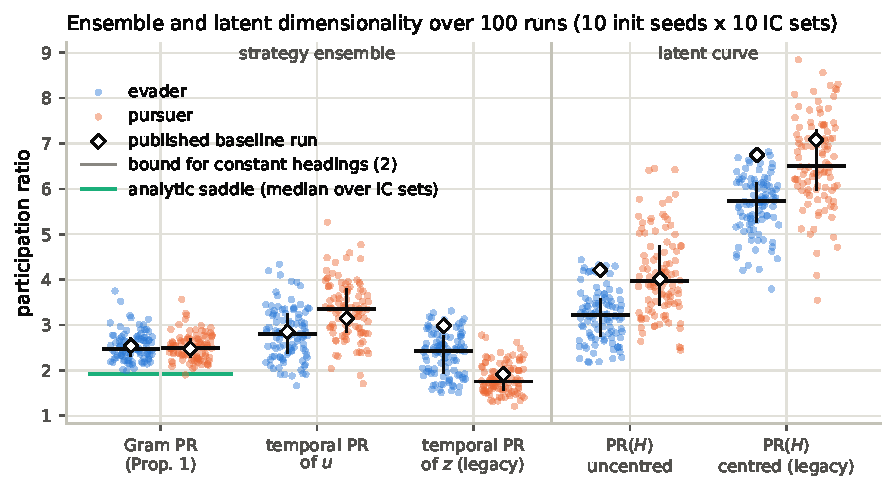
\includegraphics[width=\textwidth]{../figs/r1_dimensionalities.pdf}
\caption{Ensemble and latent dimensionality over the 100-run grid, with the published run marked. Left of the divider: gauge-invariant Gram PR and temporal PR of $\hat u$, and the legacy $\PR(Z)$. Right: latent PR, centred and uncentred.}
\label{fig:dims}
\end{figure}

\begin{figure}[t]
\centering
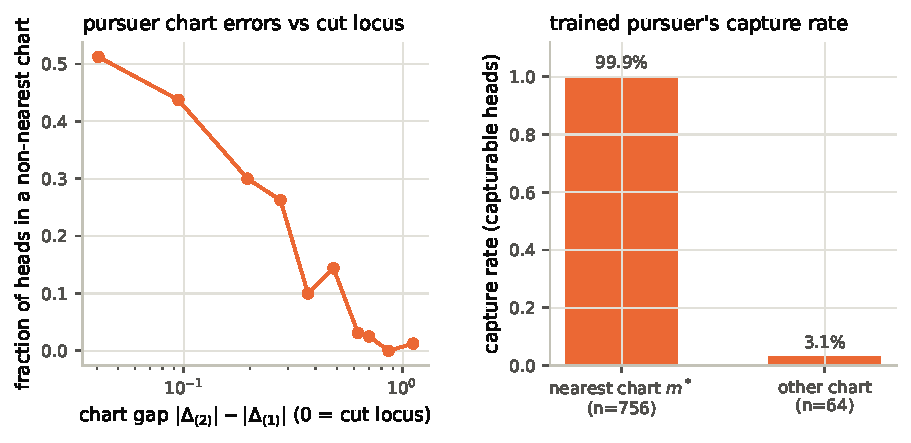
\includegraphics[width=\textwidth]{../figs/r1_charts.pdf}
\caption{Chart selection. Left: fraction of heads playing a non-nearest image chart against the chart gap $|\boldsymbol\Delta_{(2)}|-|\boldsymbol\Delta_{(1)}|$ (deciles; the gap is 0 on the cut locus). Right: the trained pursuer's capture rate on capturable heads by chart played.}
\label{fig:charts}
\end{figure}

\section*{5. Where the review agrees with the earlier evaluation}

Verified numerically: the capturable share is $\pi\cdot0.88^2/4=60.8\%$, not 59.7\%; the 4.7:1 variance ratio is not significant ($F(6,4)$, $p=0.078$); the winding label is a heading bin, not a homotopy class; Proposition~1 bounds the uncentred Gram PR, for which 2 is an upper bound, not an ideal; the run census (43 ``runs'') is 25 runs plus snapshots; C3 was trained to 15k, not 14k. Agreed on the text: \S8 is a separate study; \S9 should verify against closed-form $V^*$ and reduce the critic to a pointer; ``multi-head PINN'' is wrong because no PDE residual enters the loss; the prose needs a human rewrite from figures and tables, an abstract under 250 words, and a related-work section of about 50 references (a vetted list is in \texttt{REVIEW\_claude.md}, \S7). Not checked here: the claims about paper 2's drafts and the citation corrections (Isaacs; Melikyan--Ovakimyan 1993; Comm.\ Phys.\ 2025). One disagreement: the ``aggressive'' timeline should not keep the 8-seed baseline, because those seeds mix protocols; reruns cost about an hour.

\section*{6. Recommended changes and the remaining runs}

\begin{small}
\begin{tabularx}{\textwidth}{@{}p{2.3cm} L@{}}
\toprule
Where & Change \\
\midrule
Abstract, \S3 & Lead with: before capture, game-trained strategies are the constant-heading saddle of a jointly chosen image chart ($\eta=0.9997$, $\cos=0.99999$). Drop $\PR(Z)$; report Gram PR, $\eta$ and the temporal PR of $\hat u$ as distributions over the grid. \\
\S4 & Keep the overhead (latent temporal modes $\approx2\times$ policy modes in 99--100\% of runs) and the break at $K$; replace the init/IC split by the ANOVA; make the featurisation attribution interventional (R3). \\
\S5 & Replace the winding analysis by chart selection: misses are chart errors concentrated at the cut locus. \\
\S7 & The asymmetry is robust but post-capture; decide its mechanism (R2) before any inf--sup reading (R5). \\
\S8, \S9 & \S8 to an appendix (oracle arm stays). \S9 becomes closed-form verification: $T_c/V^*=1.01$; chart-local, fully exploitable equilibrium. \\
Throughout & One deterministic protocol; $\ge10$ runs per arm; a figure of the game, the architecture and the image charts; reproducibility stated as ``distributions reproduce''. \\
\bottomrule
\end{tabularx}
\end{small}

\medskip
Remaining runs, in order of usefulness (about 10 laptop-hours in total; each has a decision rule in \texttt{REVISION\_PLAN.md}):
\textbf{R2} capture-truncated loss, paired with R1 (tests the post-capture mechanism behind the rank excess and the asymmetry);
\textbf{R3} game-free training of the same architecture (tests ``featurisation residue'');
\textbf{R4} warm-start collapse at 10 seeds;
\textbf{R5} symmetrised protocol and single-factor ablations for the asymmetry;
\textbf{R6} $K$ and body-width sweeps;
\textbf{R7} heads sweep $N_h\in\{8,32,64,128\}$;
\textbf{R8} $\Delta v$ sweep, both players, 10 runs per value;
\textbf{R9} shaping sweep;
\textbf{R10} oracle arm and the evader side of exploitability.

\end{document}
